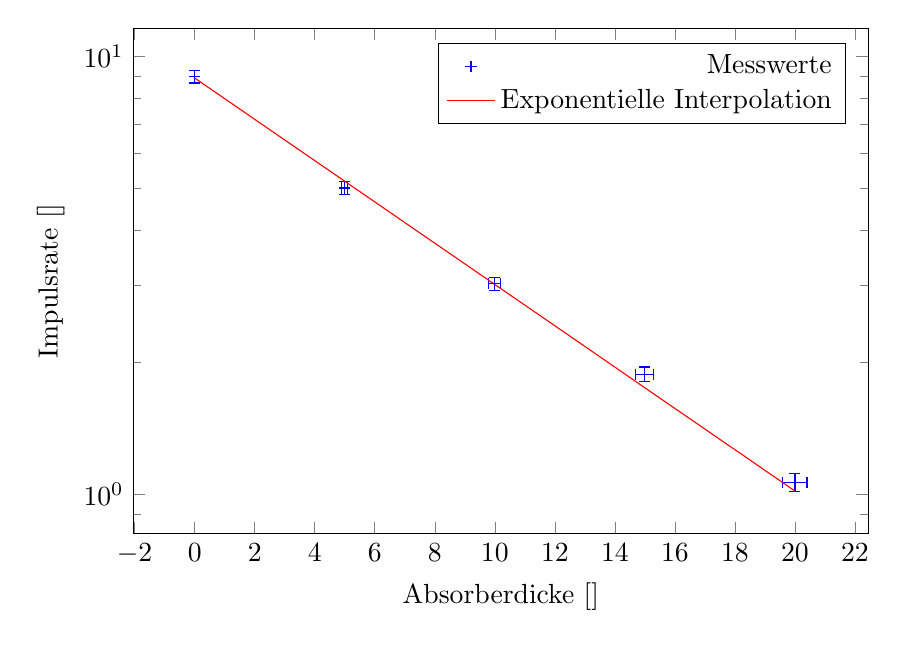
\begin{tikzpicture}
\begin{axis} [
%enlargelimits=.15,
%ybar,
%symbolic x coords={excellent, good, neutral},
%xtick = data,
width=.9\textwidth,
height = 8cm,
error bars/y dir = both,
error bars/y explicit,
%only marks,
%ymin = 0,
ymode=log,
%mark = +,
%log ticks with fixed point,
xlabel={Absorberdicke $ [\si{\milli\meter}] $},
ylabel={Impulsrate [\si{\per\second}]},
legend style = {legend pos = north east, cells={anchor=east}}
]
\addplot+[mark = +, only marks,
	error bars/x dir = both, error bars/x fixed relative=.02,] table[x = x, y= y, y error = yerror]  {
x	y	yerror
0	8.9811115104	0.2972302496
5	5.0032540334	0.1700432809
10	3.0248331846	0.1091601283
15	1.8822953388	0.0727996721
20	1.0670191931	0.0500643354
};
\addlegendentry{Messwerte}
\addplot+[no marks, domain=0:20,] 
	{8.9107847*exp(-0.10837785*x)};
\addlegendentry{Exponentielle Interpolation};
\end{axis}
\end{tikzpicture}